Una esferita $A$, electrizada positivamente, está suspendida en aire mediante un soporte y un hilo aislante. Otra esfera $B$, de masa igual a 10 g y con carga igual y opuesta a la de la esfera $A$, se coloca 10 cm abajo de ésta, como muestra la figura de este problema. En estas condiciones se encuentra que $B$ permanece en reposo al soltarla.
\begin{enumerate}
    \item ¿Cuál es el valor de la fuerza eléctrica con que $A$ atrae a $B$ (considere $g$ = 10 m/s$^2$)?
    \item ¿Cuál es la magnitud de la carga existente en cada una de las esferas?
    \item ¿Qué número de electrones hay en exceso en la esfera $B$? (Carga del electrón: $e = -1.6 \times 10^{-19}$C. Constante eléctrica: $K = 9\times 10^{-9}$Nm$^2$/C$^2$)
\end{enumerate}
\begin{figure}[h!]
  \centering
  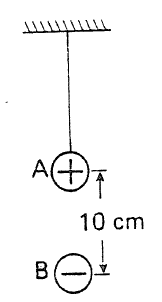
\includegraphics[scale=0.43]{figuras/fig_alvarenga_p824_12.png}
  \caption{Problema 26}
\end{figure}